\documentclass[10pt,fleqn]{article} % Default font size and left-justified equations
\usepackage[%
    pdftitle={SLCI : Transformée de Laplace},
    pdfauthor={Xavier Pessoles}]{hyperref}
%----------------------------------------------------------------------------------------
% Définition des booleéns
%----------------------------------------------------------------------------------------
\newif\iffiche
\newif\ifprof
\newif\iftd
\newif\ifcours
%\fichetrue
\fichefalse
\proftrue
%\proffalse
%\tdtrue
\tdfalse
\courstrue
%\coursfalse
%%%%%%%%%%%%%%%%%%%%%%%%%%%%%%%%%%%%%%%%%
% Original author:
% Mathias Legrand (legrand.mathias@gmail.com) with modifications by:
% Vel (vel@latextemplates.com)
% License:
% CC BY-NC-SA 3.0 (http://creativecommons.org/licenses/by-nc-sa/3.0/)
%%%%%%%%%%%%%%%%%%%%%%%%%%%%%%%%%%%%%%%%%

%----------------------------------------------------------------------------------------
%	VARIOUS REQUIRED PACKAGES AND CONFIGURATIONS
%----------------------------------------------------------------------------------------

\usepackage[top=2.5cm,bottom=2cm,left=2cm,right=2cm,headsep=40pt,a4paper]{geometry} % Page margins

\usepackage{graphicx} % Required for including pictures
\graphicspath{{images/}} % Specifies the directory where pictures are stored

\usepackage{lipsum} % Inserts dummy text

\usepackage{tikz} % Required for drawing custom shapes

\usepackage[french]{babel} % English language/hyphenation
\frenchbsetup{StandardLists=true} % Pour éviter la collision babel enumitem pour les listes

\usepackage{enumitem} % Customize lists
\setlist{nolistsep} % Reduce spacing between bullet points and numbered lists

\usepackage{booktabs} % Required for nicer horizontal rules in tables

\usepackage{xcolor} % Required for specifying colors by name
%\definecolor{ocre}{RGB}{243,102,25} % Define the orange color used for highlighting throughout the book
 \definecolor{ocre}{RGB}{49,133,156} % Couleur ''bleue''
\definecolor{violetf}{RGB}{112,48,160} % Couleur ''violet''
\usepackage{enumitem}
\usepackage{pifont} % Pour les dinglist
\usepackage{multicol}

%----------------------------------------------------------------------------------------
%	FONTS
%----------------------------------------------------------------------------------------

\usepackage{avant} % Use the Avantgarde font for headings
%\usepackage{times} % Use the Times font for headings
%\usepackage{mathptmx} % Use the Adobe Times Roman as the default text font together with math symbols from the Sym­bol, Chancery and Com­puter Modern fonts
\usepackage[adobe-utopia]{mathdesign}
\usepackage{microtype} % Slightly tweak font spacing for aesthetics
\usepackage[utf8]{inputenc} % Required for including letters with accents
\usepackage[T1]{fontenc} % Use 8-bit encoding that has 256 glyphs

%----------------------------------------------------------------------------------------
%	BIBLIOGRAPHY AND INDEX
%----------------------------------------------------------------------------------------

\usepackage[style=alphabetic,citestyle=numeric,sorting=nyt,sortcites=true,autopunct=true,babel=hyphen,hyperref=true,abbreviate=false,backref=true,backend=biber]{biblatex}
\addbibresource{bibliography.bib} % BibTeX bibliography file
\defbibheading{bibempty}{}

\usepackage{calc} % For simpler calculation - used for spacing the index letter headings correctly
\usepackage{makeidx} % Required to make an index
\makeindex % Tells LaTeX to create the files required for indexing

%----------------------------------------------------------------------------------------
%	MAIN TABLE OF CONTENTS
%----------------------------------------------------------------------------------------

\usepackage{titletoc} % Required for manipulating the table of contents

\setcounter{tocdepth}{2}     % Dans la table des matieres
\setcounter{secnumdepth}{2}

\contentsmargin{0cm} % Removes the default margin

% Part text styling
\titlecontents{part}[0cm]
{\addvspace{20pt}\centering\large\bfseries}
{}
{}
{}

% Chapter text styling
\titlecontents{chapter}[1.25cm] % Indentation
{\addvspace{12pt}\large\sffamily\bfseries} % Spacing and font options for chapters
{\color{ocre!60}\contentslabel[\Large\thecontentslabel]{1.25cm}\color{ocre}} % Chapter number
{\color{ocre}}  
{\color{ocre!60}\normalsize\;\titlerule*[.5pc]{.}\;\thecontentspage} % Page number

% Section text styling
\titlecontents{section}[1.25cm] % Indentation
{\addvspace{3pt}\sffamily\bfseries} % Spacing and font options for sections
{\color{ocre!60}\contentslabel[\thecontentslabel]{1.25cm} \color{ocre}} % Section number
{\color{ocre}}
{\hfill\color{ocre!60}\thecontentspage} % Page number
[]

% Subsection text styling
\titlecontents{subsection}[1.25cm] % Indentation
{\addvspace{1pt}\sffamily\small} % Spacing and font options for subsections
{\contentslabel[\thecontentslabel]{1.25cm}} % Subsection number
{}
{\ \titlerule*[.5pc]{.}\;\thecontentspage} % Page number
[]

% List of figures
\titlecontents{figure}[0em]
{\addvspace{-5pt}\sffamily}
{\thecontentslabel\hspace*{1em}}
{}
{\ \titlerule*[.5pc]{.}\;\thecontentspage}
[]

% List of tables
\titlecontents{table}[0em]
{\addvspace{-5pt}\sffamily}
{\thecontentslabel\hspace*{1em}}
{}
{\ \titlerule*[.5pc]{.}\;\thecontentspage}
[]

%----------------------------------------------------------------------------------------
%	MINI TABLE OF CONTENTS IN PART HEADS
%----------------------------------------------------------------------------------------

% Chapter text styling
\titlecontents{lchapter}[0em] % Indenting
{\addvspace{15pt}\large\sffamily\bfseries} % Spacing and font options for chapters
{\color{ocre}\contentslabel[\Large\thecontentslabel]{1.25cm}\color{ocre}} % Chapter number
{}  
{\color{ocre}\normalsize\sffamily\bfseries\;\titlerule*[.5pc]{.}\;\thecontentspage} % Page number

% Section text styling
\titlecontents{lsection}[0em] % Indenting
{\sffamily\small} % Spacing and font options for sections
{\contentslabel[\thecontentslabel]{1.25cm}} % Section number
{}
{}

% Subsection text styling
\titlecontents{lsubsection}[.5em] % Indentation
{\normalfont\footnotesize\sffamily} % Font settings
{}
{}
{}

%----------------------------------------------------------------------------------------
%	PAGE HEADERS
%----------------------------------------------------------------------------------------

\usepackage{fancyhdr} % Required for header and footer configuration



\pagestyle{fancy}
 \renewcommand{\headrulewidth}{0pt}
 \fancyhead{}
 \fancyhead[L]{%
 \noindent\begin{minipage}[c]{2.6cm}%
 
\includegraphics[width=4cm]{png/logo_lycee.png}%
 \end{minipage}}

\fancyhead[C]{\rule{8cm}{.5pt}}

 \fancyhead[R]{%
 \noindent\begin{minipage}[c]{3cm}
 \begin{flushright}
 \footnotesize{\textit{\textsf{\xxtete}}}%
 \end{flushright}
 \end{minipage}
}


\fancyfoot[C]{\rule{12cm}{.5pt}}
\renewcommand{\footrulewidth}{0.2pt}
\fancyfoot[C]{\footnotesize{\bfseries \thepage}}
\fancyfoot[L]{ 
\begin{minipage}[c]{.2\linewidth}
\noindent\footnotesize{{\xxauteur}}
\end{minipage}}


\fancyfoot[R]{\footnotesize{\xxpied}
\ifthenelse{\isodd{\value{page}}}{
\begin{tikzpicture}[overlay]
\node[shape=rectangle, 
      rounded corners = .25 cm,
	  draw= ocre,
	  line width=2pt, 
	  fill = ocre!10,
	  minimum width  = 2.5cm,
	  minimum height = 3cm,] at (\xxposongletx,\xxposonglety) {};
\node at (\xxposonglettext,\xxposonglety) {\rotatebox{90}{\textbf{\large\color{ocre}{\xxonglet}}}};
%{};
\end{tikzpicture}}{}
}
%
%
%
% Removes the header from odd empty pages at the end of chapters
\makeatletter
\renewcommand{\cleardoublepage}{
\clearpage\ifodd\c@page\else
\hbox{}
\vspace*{\fill}
\thispagestyle{empty}
\newpage
\fi}

\fancypagestyle{plain}{%
\fancyhf{} % vide l’en-tête et le pied~de~page.
%\fancyfoot[C]{\bfseries \thepage} % numéro de la page en cours en gras
% et centré en pied~de~page.
\fancyfoot[R]{\footnotesize{\xxpied}}
\fancyfoot[C]{\rule{12cm}{.5pt}}
\renewcommand{\footrulewidth}{0.2pt}
\fancyfoot[C]{\footnotesize{\bfseries \thepage}}
\fancyfoot[L]{ 
\begin{minipage}[c]{.2\linewidth}
\noindent\footnotesize{{\xxauteur}}
\end{minipage}}}



%----------------------------------------------------------------------------------------
%	THEOREM STYLES
%----------------------------------------------------------------------------------------

% Conflit avec la police adobe
%\usepackage{amsmath,amsfonts,amssymb,amsthm} % For math equations, theorems, symbols, etc
\usepackage{amsmath,amsthm}

\newcommand{\intoo}[2]{\mathopen{]}#1\,;#2\mathclose{[}}
\newcommand{\ud}{\mathop{\mathrm{{}d}}\mathopen{}}
\newcommand{\intff}[2]{\mathopen{[}#1\,;#2\mathclose{]}}
%\newtheorem{notation}{Notation}[chapter]
\newtheorem{notation}{Notation}[section]

% Boxed/framed environments
\newtheoremstyle{ocrenumbox}% % Theorem style name
{0pt}% Space above
{0pt}% Space below
{\normalfont}% % Body font
{}% Indent amount
{\small\bf\sffamily\color{ocre}}% % Theorem head font
{\;}% Punctuation after theorem head
{0.25em}% Space after theorem head
{\small\sffamily\color{ocre}\thmname{#1}\nobreakspace\thmnumber%{\@ifnotempty{#1}{}\@upn{#2}}% Theorem text (e.g. Theorem 2.1)
\thmnote{\nobreakspace\the\thm@notefont\sffamily\bfseries\color{black}---\nobreakspace#3.}} % Optional theorem note
\renewcommand{\qedsymbol}{$\blacksquare$}% Optional qed square


% Boite pour les corriges
\newtheoremstyle{correctionbox}% % Theorem style name
{0pt}% Space above
{0pt}% Space below
{\normalfont}% % Body font
{}% Indent amount
{\small\bf\sffamily\color{violet}}% % Theorem head font
{\;}% Punctuation after theorem head
{0.25em}% Space after theorem head
{\small\sffamily\color{ocre}\thmname{#1}\nobreakspace\thmnumber%{\@ifnotempty{#1}{}\@upn{#2}}% Theorem text (e.g. Theorem 2.1)
\thmnote{\nobreakspace\the\thm@notefont\sffamily\bfseries\color{black}---\nobreakspace#3.}} % Optional theorem note
\renewcommand{\qedsymbol}{$\blacksquare$}% Optional qed square



\newtheoremstyle{blacknumex}% Theorem style name
{5pt}% Space above
{5pt}% Space below
{\normalfont}% Body font
{} % Indent amount
{\small\bf\sffamily}% Theorem head font
{\;}% Punctuation after theorem head
{0.25em}% Space after theorem head
{\small\sffamily{\tiny\ensuremath{\blacksquare}}\nobreakspace\thmname{#1}\nobreakspace\thmnumber%{\@ifnotempty{#1}{}\@upn{#2}}% Theorem text (e.g. Theorem 2.1)
\thmnote{\nobreakspace\the\thm@notefont\sffamily\bfseries---\nobreakspace#3.}}% Optional theorem note

\newtheoremstyle{blacknumbox} % Theorem style name
{0pt}% Space above
{0pt}% Space below
{\normalfont}% Body font
{}% Indent amount
{\small\bf\sffamily}% Theorem head font
{\;}% Punctuation after theorem head
{0.25em}% Space after theorem head
{\small\sffamily\thmname{#1}\nobreakspace%\thmnumber{\@ifnotempty{#1}{}\@upn{#2}}% Theorem text (e.g. Theorem 2.1)
\thmnote{\nobreakspace\the\thm@notefont\sffamily\bfseries---\nobreakspace#3.}}% Optional theorem note

% Non-boxed/non-framed environments
\newtheoremstyle{ocrenum}% % Theorem style name
{5pt}% Space above
{5pt}% Space below
{\normalfont}% % Body font
{}% Indent amount
{\small\bf\sffamily\color{ocre}}% % Theorem head font
{\;}% Punctuation after theorem head
{0.25em}% Space after theorem head
{\small\sffamily\color{ocre}\thmname{#1}\nobreakspace\thmnumber{\@ifnotempty{#1}{}\@upn{#2}}% Theorem text (e.g. Theorem 2.1)
\thmnote{\nobreakspace\the\thm@notefont\sffamily\bfseries\color{black}---\nobreakspace#3.}} % Optional theorem note
\renewcommand{\qedsymbol}{$\blacksquare$}% Optional qed square
\makeatother

% Environnement pour les titres de parties
\newtheoremstyle{partiebox} 
{0pt}% Space above
{0pt}% Space below
{\normalfont}% Body font
{}% Indent amount
{\small\bf\sffamily}% Theorem head font
{\;}% Punctuation after theorem head
{0.25em}% Space after theorem head




% Defines the theorem text style for each type of theorem to one of the three styles above
\newcounter{dummy} 
\numberwithin{dummy}{section}
\theoremstyle{ocrenumbox}
%\newtheorem{theoremeT}[dummy]{Théorème}
\newtheorem{theoremeT}[dummy]{Théorème}
\newtheorem{resultatT}[dummy]{Résultat}
\newtheorem{objectifT}[dummy]{Objectif}
%\newtheorem{problem}{Problem}[chapter]
\newtheorem{problem}{Problem}[section]
%\newtheorem{exerciseT}{Exercise}[chapter]
\newtheorem{exerciseT}{Exercice}[section]

\theoremstyle{blacknumex}
%\newtheorem{exampleT}{Example}[chapter]
\newtheorem{exempleT}{Exemple}[section]
\theoremstyle{blacknumbox}
%\newtheorem{vocabulary}{Vocabulary}[chapter]
\newtheorem{vocabulary}{Vocabulaire}[section]
%\newtheorem{definitionT}{Definition}[section]
\newtheorem{definitionT}{Définition}[section]
\newtheorem{corollaryT}[dummy]{Corollaire}
\newtheorem{hypoT}{Hypothèse(s)}

\theoremstyle{ocrenum}
\newtheorem{proposition}[dummy]{Proposition}

\theoremstyle{partiebox}
\newtheorem{titrepartieT}[]{}
\newtheorem{titrechapitreT}[]{}

\theoremstyle{correctionbox}
\newtheorem{correctionT}[dummy]{\color{violet}{Correction}}

%----------------------------------------------------------------------------------------
%	DEFINITION OF COLORED BOXES
%----------------------------------------------------------------------------------------

\RequirePackage[framemethod=tikz]{mdframed} % Required for creating the theorem, definition, exercise and corollary boxes

% Theorem box
\newmdenv[skipabove=7pt,
skipbelow=7pt,
backgroundcolor=ocre!10,
linecolor=ocre,
innerleftmargin=5pt,
innerrightmargin=5pt,
innertopmargin=5pt,
leftmargin=0cm,
rightmargin=0cm,
innerbottommargin=5pt]{tBox}


% Correction
\newmdenv[skipabove=7pt,
skipbelow=7pt,
backgroundcolor=violet!10,
linecolor=violet,
innerleftmargin=5pt,
innerrightmargin=5pt,
innertopmargin=5pt,
leftmargin=0cm,
rightmargin=0cm,
innerbottommargin=5pt]{coBox}


% Exercise box	  
\newmdenv[skipabove=7pt,
skipbelow=7pt,
rightline=false,
leftline=true,
topline=false,
bottomline=false,
backgroundcolor=ocre!10,
linecolor=ocre,
innerleftmargin=5pt,
innerrightmargin=5pt,
innertopmargin=5pt,
innerbottommargin=5pt,
leftmargin=0cm,
rightmargin=0cm,
linewidth=4pt]{eBox}	

% Definition box
\newmdenv[skipabove=7pt,
skipbelow=7pt,
rightline=false,
leftline=true,
topline=false,
bottomline=false,
backgroundcolor=ocre!10,
linecolor=ocre,
innerleftmargin=5pt,
innerrightmargin=5pt,
innertopmargin=0pt,
leftmargin=0cm,
rightmargin=0cm,
linewidth=4pt,
innerbottommargin=0pt]{dBox}	

% Corollary box
\newmdenv[skipabove=7pt,
skipbelow=7pt,
rightline=false,
leftline=true,
topline=false,
bottomline=false,
linecolor=gray,
backgroundcolor=black!5,
innerleftmargin=5pt,
innerrightmargin=5pt,
innertopmargin=5pt,
leftmargin=0cm,
rightmargin=0cm,
linewidth=4pt,
innerbottommargin=5pt]{cBox}


% Hypothèses
\newmdenv[skipabove=7pt,
skipbelow=7pt,
rightline=false,
leftline=true,
topline=false,
bottomline=false,
linecolor=gray,
backgroundcolor=black!5,
innerleftmargin=5pt,
innerrightmargin=5pt,
innertopmargin=5pt,
leftmargin=0cm,
rightmargin=0cm,
linewidth=4pt,
innerbottommargin=5pt]{hyBox}


% Boite pour le titre de la partie (pBox)
\newmdenv[skipabove=7pt,
skipbelow=7pt,
rightline=true,
leftline=false,
topline=false,
bottomline=false,
linecolor=ocre,
backgroundcolor=none,
innerleftmargin=5pt,
innerrightmargin=5pt,
innertopmargin=5pt,
leftmargin=0cm,
rightmargin=0cm,
linewidth=4pt,
innerbottommargin=5pt]{pBox}

% Boite pour le titre du chapitre (chBox)
\newmdenv[skipabove=7pt,
skipbelow=7pt,
rightline=false,
leftline=true,
topline=false,
bottomline=false,
linecolor=ocre,
%backgroundcolor=black!5,
innerleftmargin=5pt,
innerrightmargin=5pt,
innertopmargin=5pt,
leftmargin=0cm,
rightmargin=0cm,
linewidth=4pt,
innerbottommargin=5pt]{chBox}


% Boite pour les exemples
\newmdenv[skipabove=7pt,
skipbelow=7pt,
rightline=false,
leftline=true,
topline=false,
bottomline=false,
linecolor=gray,
backgroundcolor=white,
innerleftmargin=5pt,
innerrightmargin=5pt,
innertopmargin=5pt,
leftmargin=0cm,
rightmargin=0cm,
linewidth=4pt,
innerbottommargin=5pt]{exBox}


% Creates an environment for each type of theorem and assigns it a theorem text style from the "Theorem Styles" section above and a colored box from above
\newenvironment{theorem}{\begin{tBox}\begin{theoremeT}}{\end{theoremeT}\end{tBox}}
\newenvironment{resultat}{\begin{tBox}\begin{resultatT}}{\end{resultatT}\end{tBox}}
\newenvironment{obj}{\begin{tBox}\begin{objectifT}}{\end{objectifT}\end{tBox}}
\newenvironment{corrige}{\begin{coBox}\begin{correctionT}}{\end{correctionT}\end{coBox}}
\newenvironment{exercise}{\begin{eBox}\begin{exerciseT}}{\hfill{\color{ocre}\tiny\ensuremath{\blacksquare}}\end{exerciseT}\end{eBox}}				  
\newenvironment{definition}{\begin{dBox}\begin{definitionT}}{\end{definitionT}\end{dBox}}	
\newenvironment{defi}{\begin{dBox}\begin{definitionT}}{\end{definitionT}\end{dBox}}	
%\newenvironment{exemple}{\begin{exempleT}}{\hfill{\tiny\ensuremath{\blacksquare}}\end{exempleT}}		
\newenvironment{corollary}{\begin{cBox}\begin{corollaryT}}{\end{corollaryT}\end{cBox}}
\newenvironment{hypo}{\begin{hyBox}\begin{hypoT}}{\end{hypoT}\end{hyBox}}	\newenvironment{exemple}{\begin{exBox}\begin{exempleT}}{\hfill{\tiny\ensuremath{\blacksquare}}\end{exempleT}\end{exBox}}	
\newenvironment{titrepartie}{\begin{pBox}\begin{titrepartieT}}{\end{titrepartieT}\end{pBox}}	
\newenvironment{titrechapitre}{\begin{chBox}\begin{titrechapitreT}}{\end{titrechapitreT}\end{chBox}}	
%----------------------------------------------------------------------------------------
%	REMARK ENVIRONMENT
%----------------------------------------------------------------------------------------

\newenvironment{remark}{\par\vspace{10pt}\small % Vertical white space above the remark and smaller font size
\begin{list}{}{
\leftmargin=35pt % Indentation on the left
\rightmargin=25pt}\item\ignorespaces % Indentation on the right
\makebox[-2.5pt]{\begin{tikzpicture}[overlay]
\node[draw=ocre!60,line width=1pt,circle,fill=ocre!25,font=\sffamily\bfseries,inner sep=2pt,outer sep=0pt] at (-15pt,0pt){\textcolor{ocre}{R}};\end{tikzpicture}} % Orange R in a circle
\advance\baselineskip -1pt}{\end{list}\vskip5pt} % Tighter line spacing and white space after remark

\newenvironment{rem}{\par\vspace{10pt}\small % Vertical white space above the remark and smaller font size
\begin{list}{}{
\leftmargin=35pt % Indentation on the left
\rightmargin=25pt}\item\ignorespaces % Indentation on the right
\makebox[-2.5pt]{\begin{tikzpicture}[overlay]
\node[draw=ocre!60,line width=1pt,circle,fill=ocre!25,font=\sffamily\bfseries,inner sep=2pt,outer sep=0pt] at (-15pt,0pt){\textcolor{ocre}{R}};\end{tikzpicture}} % Orange R in a circle
\advance\baselineskip -1pt}{\end{list}\vskip5pt} % Tighter line spacing and white space after remark


\newenvironment{warn}{\par\vspace{10pt}\small % Vertical white space above the remark and smaller font size
\begin{list}{}{
\leftmargin=35pt % Indentation on the left
\rightmargin=25pt}\item\ignorespaces % Indentation on the right
\makebox[-2.5pt]{\begin{tikzpicture}[overlay]
\node[draw=red!60,line width=1pt,circle,fill=red!25,font=\sffamily\bfseries,inner sep=2pt,outer sep=0pt] at (-15pt,0pt){\textcolor{black}{!}};\end{tikzpicture}} % Point d'exclamation dans un cercle
\advance\baselineskip -1pt}{\end{list}\vskip5pt} % Tighter line spacing and white space after remark


%----------------------------------------------------------------------------------------
%	SECTION NUMBERING IN THE MARGIN
%----------------------------------------------------------------------------------------

\makeatletter
\renewcommand{\@seccntformat}[1]{\llap{\textcolor{ocre}{\csname the#1\endcsname}\hspace{1em}}}                    
\renewcommand{\section}{\@startsection{section}{1}{\z@}
{-4ex \@plus -1ex \@minus -.4ex}
{1ex \@plus.2ex }
{\normalfont\large\sffamily\bfseries}}
\renewcommand{\subsection}{\@startsection {subsection}{2}{\z@}
{-3ex \@plus -0.1ex \@minus -.4ex}
{0.5ex \@plus.2ex }
{\normalfont\sffamily\bfseries}}
\renewcommand{\subsubsection}{\@startsection {subsubsection}{3}{\z@}
{-2ex \@plus -0.1ex \@minus -.2ex}
{.2ex \@plus.2ex }
{\normalfont\small\sffamily\bfseries}}                        
\renewcommand\paragraph{\@startsection{paragraph}{4}{\z@}
{-2ex \@plus-.2ex \@minus .2ex}
{.1ex}
{\normalfont\small\sffamily\bfseries}}

%----------------------------------------------------------------------------------------
%	PART HEADINGS
%----------------------------------------------------------------------------------------


%----------------------------------------------------------------------------------------
%	CHAPTER HEADINGS
%----------------------------------------------------------------------------------------

% \newcommand{\thechapterimage}{}%
% \newcommand{\chapterimage}[1]{\renewcommand{\thechapterimage}{#1}}%
% \def\@makechapterhead#1{%
% {\parindent \z@ \raggedright \normalfont
% \ifnum \c@secnumdepth >\m@ne
% \if@mainmatter
% \begin{tikzpicture}[remember picture,overlay]
% \node at (current page.north west)
% {\begin{tikzpicture}[remember picture,overlay]
% \node[anchor=north west,inner sep=0pt] at (0,0) {\includegraphics[width=\paperwidth]{\thechapterimage}};
% \draw[anchor=west] (\Gm@lmargin,-9cm) node [line width=2pt,rounded corners=15pt,draw=ocre,fill=white,fill opacity=0.5,inner sep=15pt]{\strut\makebox[22cm]{}};
% \draw[anchor=west] (\Gm@lmargin+.3cm,-9cm) node {\huge\sffamily\bfseries\color{black}\thechapter. #1\strut};
% \end{tikzpicture}};
% \end{tikzpicture}
% \else
% \begin{tikzpicture}[remember picture,overlay]
% \node at (current page.north west)
% {\begin{tikzpicture}[remember picture,overlay]
% \node[anchor=north west,inner sep=0pt] at (0,0) {\includegraphics[width=\paperwidth]{\thechapterimage}};
% \draw[anchor=west] (\Gm@lmargin,-9cm) node [line width=2pt,rounded corners=15pt,draw=ocre,fill=white,fill opacity=0.5,inner sep=15pt]{\strut\makebox[22cm]{}};
% \draw[anchor=west] (\Gm@lmargin+.3cm,-9cm) node {\huge\sffamily\bfseries\color{black}#1\strut};
% \end{tikzpicture}};
% \end{tikzpicture}
% \fi\fi\par\vspace*{270\p@}}}

%-------------------------------------------

\def\@makeschapterhead#1{%
\begin{tikzpicture}[remember picture,overlay]
\node at (current page.north west)
{\begin{tikzpicture}[remember picture,overlay]
\node[anchor=north west,inner sep=0pt] at (0,0) {\includegraphics[width=\paperwidth]{\thechapterimage}};
\draw[anchor=west] (\Gm@lmargin,-9cm) node [line width=2pt,rounded corners=15pt,draw=ocre,fill=white,fill opacity=0.5,inner sep=15pt]{\strut\makebox[22cm]{}};
\draw[anchor=west] (\Gm@lmargin+.3cm,-9cm) node {\huge\sffamily\bfseries\color{black}#1\strut};
\end{tikzpicture}};
\end{tikzpicture}
\par\vspace*{270\p@}}
\makeatother

%----------------------------------------------------------------------------------------
%	HYPERLINKS IN THE DOCUMENTS
%----------------------------------------------------------------------------------------


\hypersetup{hidelinks,backref=true,pagebackref=true,hyperindex=true,colorlinks=false,breaklinks=true,urlcolor= ocre,bookmarks=true,bookmarksopen=false,pdftitle={Title},pdfauthor={Author}}
\usepackage{bookmark}
\bookmarksetup{
open,
numbered,
addtohook={%
\ifnum\bookmarkget{level}=0 % chapter
\bookmarksetup{bold}%
\fi
\ifnum\bookmarkget{level}=-1 % part
\bookmarksetup{color=ocre,bold}%
\fi
}
}

%----------------------------------------------------------------------------------------
%	
%----------------------------------------------------------------------------------------

\newcommand{\thechapterimage}{}%
\newcommand{\chapterimage}[1]{\renewcommand{\thechapterimage}{#1}}%
\def\@makechapterhead#1{%
{\parindent \z@ \raggedright \normalfont
\begin{tikzpicture}[remember picture,overlay]
\node at (current page.north west)
{\begin{tikzpicture}[remember picture,overlay]
\node[anchor=north west,inner sep=0pt] at (0,0) {\includegraphics[width=\paperwidth]{\thechapterimage}};
%\draw[anchor=west] (\Gm@lmargin,-9cm) node [line width=2pt,rounded corners=15pt,draw=ocre,fill=white,fill opacity=0.5,inner sep=15pt]{\strut\makebox[22cm]{}};
%\draw[anchor=west] (\Gm@lmargin+.3cm,-9cm) node {\huge\sffamily\bfseries\color{black}\thechapter. #1\strut};
\end{tikzpicture}};
\end{tikzpicture}
\par\vspace*{270\p@}
}}




\makeatletter             
\renewcommand{\subparagraph}{\@startsection{subparagraph}{5}{\z@}%
                                    {-2ex \@plus-.2ex \@minus .2ex}%
                                    {0ex}%               
{\normalfont\bfseries Question \hspace{.7cm} }}
\makeatother
\renewcommand{\thesubparagraph}{\arabic{subparagraph}} 
\makeatletter


% Définition des booleéns
\newif\iffiche
\newif\ifprof
\newif\iftd
\newif\ifcours

%%%%%%%%%%%%
% Par coeur, a faire, correction  
%%%%%%%%%%%%

\usepackage{pifont}% http://ctan.org/pkg/pifont
\newcommand{\cmark}{\color{green}\ding{51}}%
\newcommand{\xmark}{\color{red}\ding{55}}%
\newcommand{\fmark}{\ding{229}}%
\newcommand{\itemc}{\item[\cmark]}%
\newcommand{\itemx}{\item[\xmark]}%
\newcommand{\itemf}{\item[\fmark]}%

\newcommand{\parcoeur}{{\large\ding{164}} }
\newcommand{\afaire}{{\large\ding{46}} }
\newcommand{\correction}{{\large\ding{52}} }

\usepackage{array}
\newcolumntype{P}[1]{>{\centering\arraybackslash}p{#1}}
%%%%%%%%%%%%
% Définition des vecteurs 
%%%%%%%%%%%%
 \newcommand{\vect}[1]{\overrightarrow{#1}}
\newcommand{\axe}[2]{\left(#1,\vect{#2}\right)}

\newcommand{\rep}[1]{\mathcal{R}_{#1}}
\newcommand{\vx}[1]{\vect{x_{#1}}}
\newcommand{\vy}[1]{\vect{y_{#1}}}
\newcommand{\vz}[1]{\vect{z_{#1}}}

%%%%%%%%%%%%
% Définition des torseurs 
%%%%%%%%%%%%

 \newcommand{\torseur}[1]{%
\left\{{#1}\right\}
}

\newcommand{\torseurcin}[3]{%
\left\{\mathcal{#1} \left(#2/#3 \right) \right\}
}

\newcommand{\torseurstat}[3]{%
\left\{\mathcal{#1} \left(#2\rightarrow #3 \right) \right\}
}

 \newcommand{\torseurc}[8]{%
%\left\{#1 \right\}=
\left\{
{#1}
\right\}
 = 
\left\{%
\begin{array}{cc}%
{#2} & {#5}\\%
{#3} & {#6}\\%
{#4} & {#7}\\%
\end{array}%
\right\}_{#8}%
}

 \newcommand{\torseurcol}[7]{
\left\{%
\begin{array}{cc}%
{#1} & {#4}\\%
{#2} & {#5}\\%
{#3} & {#6}\\%
\end{array}%
\right\}_{#7}%
}

 \newcommand{\torseurl}[3]{%
%\left\{\mathcal{#1}\right\}_{#2}=%
\left\{%
\begin{array}{l}%
{#1} \\%
{#2} %
\end{array}%
\right\}_{#3}%
}

 \newcommand{\vectv}[3]{%
\vect{V\left( {#1} \in {#2}/{#3}\right)}
}


\newcommand{\vectf}[2]{%
\vect{R\left( {#1} \rightarrow {#2}\right)}
}

\newcommand{\vectm}[3]{%
\vect{\mathcal{M}\left( {#1}, {#2} \rightarrow {#3}\right)}
}


 \newcommand{\vectg}[3]{%
\vect{\Gamma \left( {#1} \in {#2}/{#3}\right)}
}

 \newcommand{\vecto}[2]{%
\vect{\Omega\left( {#1}/{#2}\right)}
}
% }$$\left\{\mathcal{#1} \right\}_{#2} =%
% \left\{%
% \begin{array}{c}%
%  #3 \\%
%  #4 %
% \end{array}%
% \right\}_{#5}}
%% Ça, ce sont les commandes publiques %%
\newcommand{\RemplirTrou}{false}
\newcommand{\TailleTrou}{\Large}
\newcommand{\ColorTrou}{black}
\newlength{\DeltaTrou}
\setlength{\DeltaTrou}{0pt}
%%%%%%%%%%%%%%%%%%%%%%%%%%%%%%%%%%%%%%%%%

\newsavebox{\totoTrou}
\newsavebox{\tataTrou}
\newlength{\longpointTrou}
\newlength{\profondeurTrou}
\newlength{\hauteurTrou}


\newcommand{\trou}[2][\RemplirTrou]{%
    \savebox{\tataTrou}{\hbox{\color{\ColorTrou}.}}%
    \leavevmode%
    \ifthenelse{\equal{#1}{false}}{%
        \ifmmode%
            \ifinner%
                \savebox{\totoTrou}{\TailleTrou$#2$}%
                \settodepth{\profondeurTrou}{\TailleTrou$#2$}%
                \settoheight{\hauteurTrou}{\TailleTrou$#2$}%
            \else%
                \savebox{\totoTrou}{\TailleTrou$\displaystyle#2$}%
                \settodepth{\profondeurTrou}{\TailleTrou$\displaystyle#2$}%
                \settoheight{\hauteurTrou}{\TailleTrou$\displaystyle#2$}%
            \fi%
        \else%
            \savebox{\totoTrou}{\TailleTrou#2}%
                \settodepth{\profondeurTrou}{\TailleTrou#2}%
                \settoheight{\hauteurTrou}{\TailleTrou#2}%
        \fi%
        \setlength{\longpointTrou}{0pt}%
        \whiledo{\longpointTrou<\wd\totoTrou}{%
            \hbox{%\TailleTrou%\rule{0pt}{\baselineskip}% <-- version d'origine
                  \rule[-\profondeurTrou-\DeltaTrou]{0pt}{\profondeurTrou+\hauteurTrou+2\DeltaTrou}% <-- ma version
                  \usebox{\tataTrou}%
            }% fin de \hbox
            \penalty0\advance\longpointTrou by\wd\tataTrou%
        }% fin du whiledo
    }% fin du then de ifthenelse
    {%
        {\textbf{\color{red}#2}}%
    }% fin du else de ifthenelse
}% fin de la définition de \trou


\usepackage{siunitx}
% -------------------------------------
% Déclaration des titres
% -------------------------------------

\def\discipline{Enseignement \\Technologique \\ Transversal}
\def\xxtete{Enseignement Technologique Transversal}

\def\classe{1 STI2D}
\def\xxnumpartie{Seq 3}
\def\xxpartie{Alimenter un système en énergie}

\def\xxnumchapitre{Séance 1}
\def\xxchapitre{\hspace{.12cm} La fonction alimenter/stocker}

\def\xxposongletx{2}
\def\xxposonglettext{1.45}
\def\xxposonglety{23}
\def\xxonglet{Seq. 3 -- Se. 1}

\def\xxactivite{Cours}
\def\xxauteur{\textsl{Geoffrey Vaquette}}

\def\xxcompetences{%
\textsl{%
\textbf{Savoirs et compétences :}
\begin{itemize}[label=\ding{112},font=\color{ocre}]
\item CO2.1	Identifier les flux et la forme de l'énergie, caractériser ses transformations et/ou modulations et estimer l'efficacité globale d'un système.
\end{itemize}
%
}}

\def\xxfigures{
\begin{center}
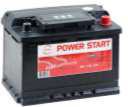
\includegraphics[width=2cm]{images/batterie.png} \\
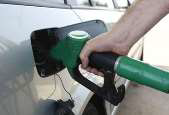
\includegraphics[width=2cm]{images/essence.png} \\
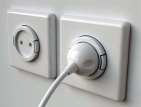
\includegraphics[width=2cm]{images/prise.png} \\
\end{center}
}%figues de la page de garde
\def\xxpied{%
La fonction alimenter/stocker \xxactivite%
}

%---------------------------------------------------------------------------

\renewcommand{\RemplirTrou}{false}
\begin{document}
\chapterimage{images/stockage_energie.jpg}
\pagestyle{empty}


%\chapterentete{}

\iftd
\begin{tikzpicture}[remember picture,overlay]
\node at (current page.north west)
{\begin{tikzpicture}[remember picture,overlay]
\draw[anchor=west] (-2cm,-3.25cm) node [line width=2pt,rounded corners=15pt,draw=ocre,fill=white,fill opacity=0.6,inner sep=40pt]{\strut\makebox[22cm]{}};
\draw[anchor=west] (1cm,-3.25cm) node {\huge\sffamily\bfseries\color{black} %
\begin{minipage}{1cm}
\rotatebox{90}{\LARGE\sffamily\textsc{\color{ocre}\textbf{\xxnumpartie}}}
\end{minipage} \hfill
\begin{minipage}[c]{13.5cm}
\begin{titrepartie}
\begin{flushright}
\renewcommand{\baselinestretch}{1.1} 
\Large\sffamily\textsc{\textbf{\xxpartie}}
\renewcommand{\baselinestretch}{1} 
\end{flushright}
\end{titrepartie}
\end{minipage} \hfill
\begin{minipage}[c]{3.5cm}
{\large\sffamily\textsc{\textbf{\color{ocre} \discipline}}}
\end{minipage} 
 };
\end{tikzpicture}};
\end{tikzpicture}


\else
\begin{tikzpicture}[remember picture,overlay]
\node at (current page.north west)
{\begin{tikzpicture}[remember picture,overlay]
\node[anchor=north west,inner sep=0pt] at (0,0) {\includegraphics[width=\paperwidth, height=5cm]{\thechapterimage}};
\draw[anchor=west] (-2cm,-8cm) node [line width=2pt,rounded corners=15pt,draw=ocre,fill=white,fill opacity=0.6,inner sep=40pt]{\strut\makebox[22cm]{}};
\draw[anchor=west] (1cm,-8cm) node {\huge\sffamily\bfseries\color{black} %
\begin{minipage}{1cm}
\rotatebox{90}{\LARGE\sffamily\textsc{\color{ocre}\textbf{\xxnumpartie}}}
\end{minipage} \hfill
\begin{minipage}[c]{14cm}
\begin{titrepartie}
\begin{flushright}
\renewcommand{\baselinestretch}{1.1} 
\Large\sffamily\textsc{\textbf{\xxpartie}}
\renewcommand{\baselinestretch}{1} 
\end{flushright}
\end{titrepartie}
\end{minipage} \hfill
\begin{minipage}[c]{3.5cm}
{\large\sffamily\textsc{\textbf{\color{ocre} \discipline}}}
\end{minipage} 
 };
\end{tikzpicture}};
\end{tikzpicture}

\fi



% Chapitre + TABLE DES MATIERES(dans le cas du cours)
\iftd
\vfill
\begin{tikzpicture}[overlay]
\node[shape=rectangle, 
      rounded corners = .25 cm,
	  draw= ocre,
	  line width=2pt, 
	  fill = ocre!10,
	  minimum width  = 2.5cm,
	  minimum height = 3cm,] at (18cm,0) {};
\node at (17.7cm,0) {\rotatebox{90}{\textbf{\Large\color{ocre}{\classe}}}};
%{};
\end{tikzpicture}

\vspace {3.5 cm}

\begin{tikzpicture}[remember picture,overlay]
\draw[anchor=west] (-2cm,-6cm) node {\huge\sffamily\bfseries\color{black} %
\begin{minipage}{2cm}
\LARGE\sffamily\textsc{\color{ocre}\textbf{\xxactivite}}
\end{minipage} \hfill
\begin{minipage}[c]{15cm}
\begin{titrechapitre}
\renewcommand{\baselinestretch}{1.1} 
\Large\sffamily\textsc{\textbf{\xxnumchapitre}}

\Large\sffamily\textsc{\textbf{\xxchapitre}}
\vspace{.5cm}

\renewcommand{\baselinestretch}{1} 
\normalsize\normalfont
\xxcompetences
\end{titrechapitre}
\end{minipage}  };
\end{tikzpicture}

\else


\begin{tikzpicture}[overlay]
\node[shape=rectangle, 
      rounded corners = .25 cm,
	  draw= ocre,
	  line width=2pt, 
	  fill = ocre!10,
	  minimum width  = 2.5cm,
	  minimum height = 3cm,] at (18cm,0) {};
\node at (17.7cm,0) {\rotatebox{90}{\textbf{\Large\color{ocre}{\classe}}}};
%{};
\end{tikzpicture}

\vspace{3.5cm}

\begin{tikzpicture}[remember picture,overlay]
\draw[anchor=west] (-2cm,-6cm) node {\huge\sffamily\bfseries\color{black} %
\begin{minipage}{2cm}
\LARGE\sffamily\textsc{\color{ocre}\textbf{\xxactivite}}
\end{minipage} \hfill
\begin{minipage}[c]{15cm}
\begin{titrechapitre}
\renewcommand{\baselinestretch}{1.1} 
\Large\sffamily\textsc{\textbf{\xxnumchapitre}}

\Large\sffamily\textsc{\textbf{\xxchapitre}}
\vspace{.5cm}

\renewcommand{\baselinestretch}{1} 
\normalsize\normalfont
\xxcompetences
\end{titrechapitre}
\end{minipage}  };
\end{tikzpicture}
\vfill

\begin{flushright}
\begin{minipage}[c]{.3\linewidth}
\begin{center}
\xxfigures
\end{center}
\end{minipage}\hfill
\begin{minipage}[c]{.6\linewidth}
\startcontents
\printcontents{}{1}{}
\end{minipage}
\end{flushright}

\begin{tikzpicture}[remember picture,overlay]
\draw[anchor=west] (4.5cm,-.7cm) node {
\begin{minipage}[c]{.2\linewidth}
\begin{flushright}

\includegraphics[width=2cm]{../png/logoCC}
\end{flushright}
\end{minipage}
\begin{minipage}[c]{.2\linewidth}
\textsl{\xxauteur} \\
\textsl{\classe}
\end{minipage}
 };
\end{tikzpicture}
\newpage
\pagestyle{fancy}
\fi
\section{Généralités}
\subsection{Définition}
Tout système nécessite de l’énergie pour fonctionner (pour agir sur la matière d'oeuvre). Dans la chaîne d’énergie, la fonction qui permet de fournir l’énergie est la fonction « Alimenter/Stocker ».

Nous nous intéresserons particulièrement dans ce cours à ce premier bloc de la chaîne d'énergie. 

\begin{defi}
    Les éléments du bloc \textbf{Alimenter/Stocker} ont pour fonction de fournir l'énergie au système. Cette énergie peut provenir de l'extérieur du système (Réseau électrique par exemple) ou être stockée au sein du système (Batterie électrique par exemple). 
\end{defi}


\subsection{Pourquoi stocker de l'énergie ?}
Le stockage de l'énergie est utilisé pour répondre à trois besoins principaux : 
\begin{description}
    \item[Autonomie : ] Rendre un système mobile, capable de se déplacer avec sa source d'énergie.
    \begin{itemize}
        \item Voitures
        \item Téléphones 
        \item Avion
        \item \dots
    \end{itemize}
    \item[Décalage temporel : ] Il n'est pas toujours possible de générer de l'énergie au moment où elle doit être utilisée. Par exemple, une maison équipée en panneau solaire ne pourrait pas être éclairée la nuit sans stockage de l'énergie.  
    \item[Compensation des fluctuations : ]Il peut exister des fluctuations de courant électrique non désirées. Ces fluctuations peuvent être compensées par une réserve d'énergie. 
\end{description}

\section{Stoker de l'énergie électrique}
L'énergie électrique est l'énergie la plus utilisée par l'être humain dans la société actuelle. Cette énergie provient de centrales à énergie renouvelables, ou non-renouvelables. 

Il est aujourd'hui \textbf{impossible} de stocker de l'énergie sous forme électrique. Pour stocker cette énergie, il est donc indispensable de la convertir. 

\subsection{Stockage chimique : piles et batterie}
Les piles et les batteries sont les principaux dispositifs que nous côtoyons au quotidien pour stocker de l'énergie. 
L'énergie électrique est stockée dans des piles sous forme d'énergie chimique. Ces composants ont un coup abordable mais souvent un impact environnemental relativement fort. 

\subsubsection{Caractéristiques des piles et batteries}
Les batteries sont caractérisées par trois grandeurs principales : 
\begin{description}
    \item[La tension :] Classiquement notée $U$, la tension d'une batterie est la différence de potentiel qu'elle impose à ses bornes lors de sa décharge. Elle s'exprime en \textbf{volts (V)}
    
    \item[La capacité : ] C'est la quantité d'électricité (ou nombre de charges) stockée dans la batterie. Elle est habituellement indiquée en \textbf{ampère-heure (Ah)} ou en \textbf{Coulomb (C)}.
    
    \item[La densité énergétique : ]C'est la quantité d'énergie par unité de masse ou de volume. Elle s'exprime en \SI{Wh}{kg} ou \SI{Wh}{L}
    
\end{description}

\begin{table}[]
    \centering
    \begin{tabular}{>{\centering\arraybackslash} m{3cm}|>{\centering\arraybackslash} m{2cm}|>{\centering\arraybackslash} m{2cm}|>{\centering\arraybackslash} m{2cm}|>{\centering\arraybackslash} m{6cm}}
        \textbf{Type de batterie} & \textbf{Densité (\si{Wh/kg})} & \textbf{Plage de puissance} & \textbf{Rendement} & \textbf{Utilisation}  \\\hline
        Plomb & 50 & \SI{100}{W} à \SI{10}{MW} & 70 à 85 \% & \begin{itemize}
            \item Véhicules routiers électriques
            \item Sites non raccordés au réseau
        \end{itemize}\\\hline
        NiCd : Nickel-Cadmium& 50&Quelques Watts&70 à 80\%&\begin{itemize}
            \item Outillages portatifs
            \item Rasoirs électriques
        \end{itemize}\\\hline
        NiMH : Nickel Métal Hydrure&75&Quelques Watts&70 à 80\%&\begin{itemize}
            \item Téléphones portables
            \item Appareils photos
            \item Rasoirs électriques
        \end{itemize} \\\hline
        Li-ion : Lithium-ion&300&50W à 10MW&85 à 90\%& \begin{itemize}
            \item Téléphones portables
            \item Véhicules électriques
            \item Appareils photo
            \item Ordinateurs portables
        \end{itemize}\\\hline
        Li-Pol : Lithium-Polymère&120&100W à 10MW&85 à 90\%&\begin{itemize}
            \item Téléphones portables
            \item Véhicules électriques légers
        \end{itemize}
    \end{tabular}
    
    \caption{Quelques technologies de batteries.}
    \label{tab:my_label}
\end{table}

\begin{warn}
    Attention, il est important de ne pas confondre l'intensité (en \si{A}) et la capacité (en \si{Ah}).
\end{warn}

\begin{warn}
    La capacité d'une batterie ne représente pas directement la quantité d'énergie qu'elle contient. Pour connaître la quantité d'énergie contenue dans une batterie, il faut \textbf{multiplier sa capacité par sa tension} $$E = C \times U$$.
\end{warn}

\begin{rem}
        Une batterie contenant 10Ah sera capable de fournir un courant de 10A pendant 1h, ou encore un courant de 5A pendant 2h. 
\end{rem}

\begin{exemple}
    Calculer la quantité d'énergie contenue dans une batterie d'une tension de $U = \SI{3}{V}$, d'une capacité de $Ca=\SI{1.5}{Ah}$.
\end{exemple}
\begin{correction}
     \trou{Une capacité de $C_a= \SI{1.5}{Ah}$ équivaut à une quantité de charges $q = Ca \times 3600 = \SI{5400}{C}$}
\end{correction}

\subsubsection{Association de batteries}

\begin{figure}[h]
    \centering
    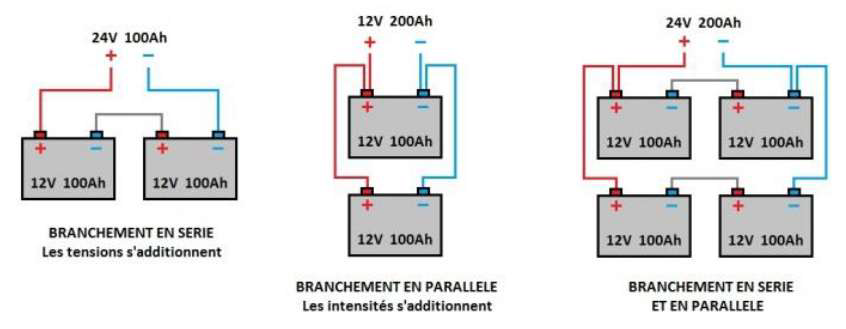
\includegraphics[width=\textwidth]{images/association.png}
    \caption{Association de batteries}
    \label{fig:association}
\end{figure}


\subsubsection{Synthèse : }
    \begin{aretenir}~
            \begin{itemize}
                \item Un courant électrique est un déplacement de charges (électrons).
                \item La quantité d'électricité $q$ (en coulomb \si{C}) est le produit de l'intensité \textbf{I} en \si{A} par le temps \textbf{t} en \si{s}. 
                \item On peut également exprimer une quantité d'électricité $q$ en Ampère-heure (\si{Ah}).
            \end{itemize}
            \vspace{0.2cm}
        ~\hfill\fbox{\large$q = I\times t$}\hfill\fbox{\large$\SI{1}{Ah} = \SI{3600}{C}$}\hfill~
    \end{aretenir}
    
    \begin{aretenir}
        La puissance consommée $P$ en \si{W} est égale au produit de la tension \textbf{U} (en \si{V})  par le courant \textit{I} (en A) qui circule.
        
        \begin{center}
            \fbox{\large$P = U\times I$}
        \end{center}
        
    \end{aretenir}
    
    \begin{aretenir}
        L'énergie $E$ fournie par une batterie est : 
        \begin{itemize}
            \item égale au produit de la \textbf{puissance absorbée} (en \si{W}) par le \textbf{temps de fonctionnement}
            \begin{itemize}
                \item Si t est en secondes \si{s}, E est en \si{J}
                \item Si t est en heures \si{h}, E est en \si{Wh}
            \end{itemize}
            \begin{center}
                \fbox{\large$E = P \times t$}
            \end{center}
            
            \item égale au produit de la capacité de la batterie par la tension ($\si{Ah}\times\si{V} = Wh$: 
            \begin{center}
                \fbox{E=C\times U}
            \end{center}
        \end{itemize}
    \end{aretenir}
    
    \subsection{Stockage hydrolique}
    
    A plus grande échelle, on stocke de l'eau à l'aide de bassins de rétention : 
    \begin{itemize}
        \item Lorsque l'on produit globalement plus d'énergie que la demande, on actionne des pompes pour faire monter l'eau dans un bassin en altitude. 
        \item Lorsque l'on produit globalement \textbf{moins} d'énergie que la demande, on produit de l'électricité en faisant descendre l'eau dans des conduites pour activer des turbines. 
    \end{itemize}
    
    \begin{figure}[h]
        \centering
        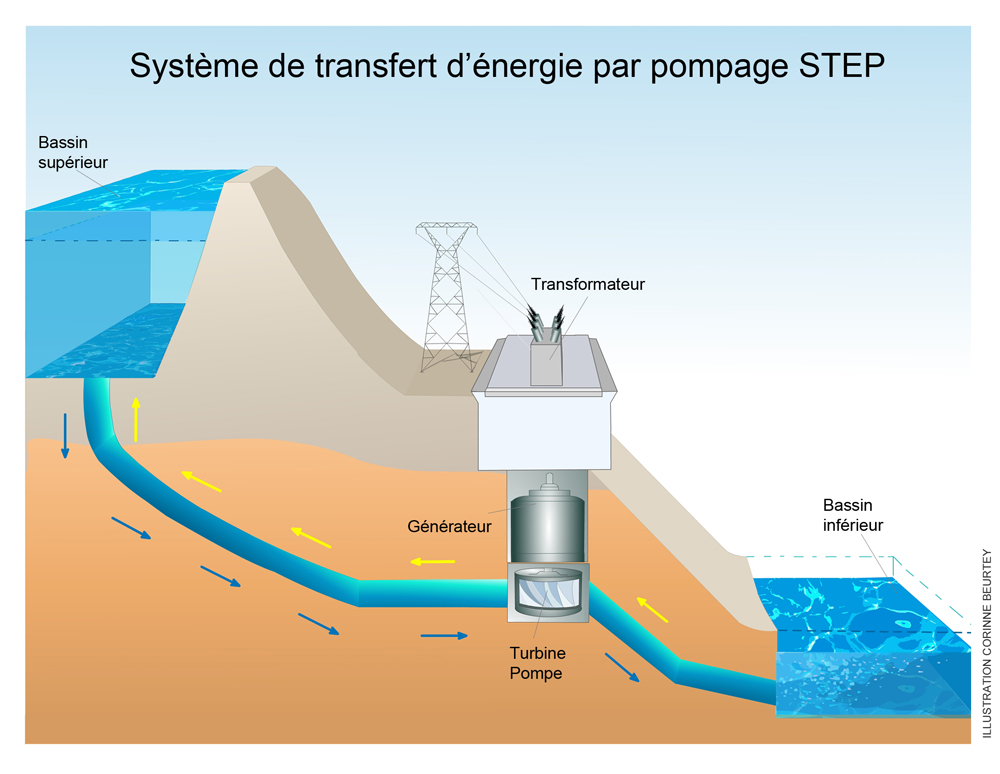
\includegraphics[width=\textwidth]{images/hydrau}
        \caption{Système de stockage d'énergie}
        \label{fig:hydrau}
    \end{figure}
    
    
    \section{Les signaux électriques}
    L'énergie électrique peut circuler sous différentes formes de signaux. Nous décrivons dans cette section les caractéristiques d'un signal électrique. 
    
    \subsection{Les signaux périodiques}
    
    \begin{defi}
        Un signal est dit périodique si les variations de son amplitude se reproduisent régulièrement au bout d'une période \textbf{T} constante.
        
        \begin{center}
            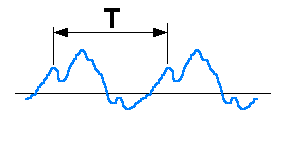
\includegraphics[width=0.3\textwidth]{images/Signal_periodique.png}
        \end{center}
        
        On a u(t+T) = u(t)
    \end{defi}
    
    \subsubsection{Caractéristiques d'un signal périodique}
    \begin{aretenir}~
    \begin{description}
        \item[La période T :] C'est la durée entre deux instants où la grandeur se reproduit identiquement à elle-même. La période s'exprime en \si{s}.
        
        \item[La fréquence f :] C'est le nombre de périodes présentes dans chaque seconde. Elle s'exprime en \si{Hz} est vaut : 
        \begin{center}
            \fbox{$f = \frac{1}{T}$}
        \end{center}
        \item[Les valeurs maximales $S_{\text{max}}$ et minimales $S_{\text{min}}$] sont respectivement le maximum et le minimum du signal.
        \item[L'amplitude crête à crête S_{CC}] est l'écart entre les valeurs maximale et minimale : \fbox{$S_{CC} = S_{\text{max}} - S_\text{min}$}
        \item[L'amplitude A :] \fbox{$A = \frac{S_{CC}}{2}$}
        \item[Valeur efficace $S_\text{eff}$ : ] Elle est égale à la tension continue qu'il faudrait appliquer à une lampe pour qu'elle ait la même luminosité qu'avec une tension périodique.
    \end{description}
    \end{aretenir}
    
    \subsubsection{Le signal sinusoïdal}
    Le signal sinusoïdal est le type de signal le plus répandu dans les réseau électrique. Il a la forme d'une sinusoïde : $S = A\sin{\omega t} + S_\text{moy}$
    
    \begin{center}
        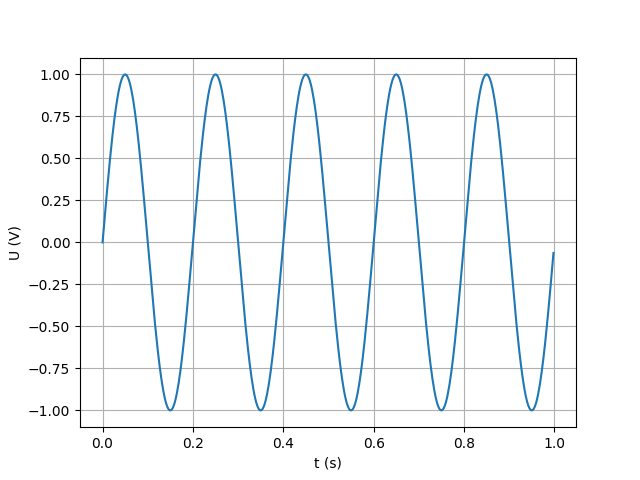
\includegraphics[height=0.3\textheight]{images/sinus.png}
    \end{center}
    \begin{itemize}
        \item La période de ce signal vaut : \trou{$T = \SI{0.2}{s}$}
        \item La fréquence de ce signal vaut : \trou{$f = \frac{1}{T}\SI{5}{Hz}$}
        \item  L'amplitude de ce signal vaut : \trou{$A = 1V$}
    \end{itemize}
        
        
       
    
    \subsubsection{Le signal carré}
    Un signal carré est généralement employé pour transporter une information ou pour commander un moteur à courant continu. 
    \begin{center}
        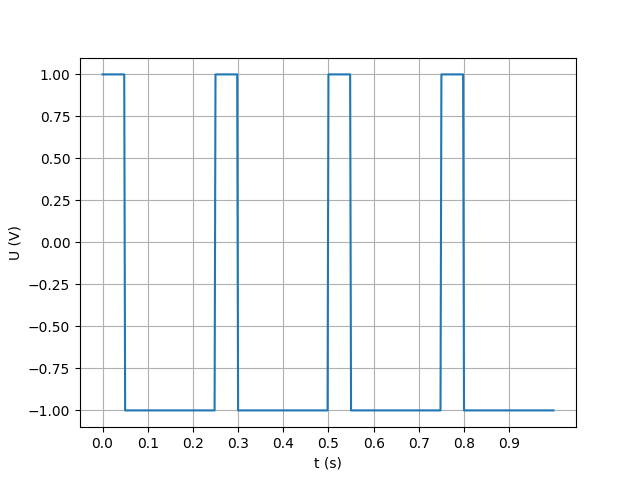
\includegraphics[height=0.3\textheight]{images/carre.png}
    \end{center}
    
    \begin{defi}
        Le rapport cyclique $\alpha$ d'un signal carré est le temps resté à l'état haut divisé par la période du signal. 
    \end{defi}
    
    \begin{exemple}
        Le rapport cyclique de ce signal vaut : \trou{0.3}
    \end{exemple}
    
    
    \subsubsection{Le signal triangulaire}
    \begin{center}
        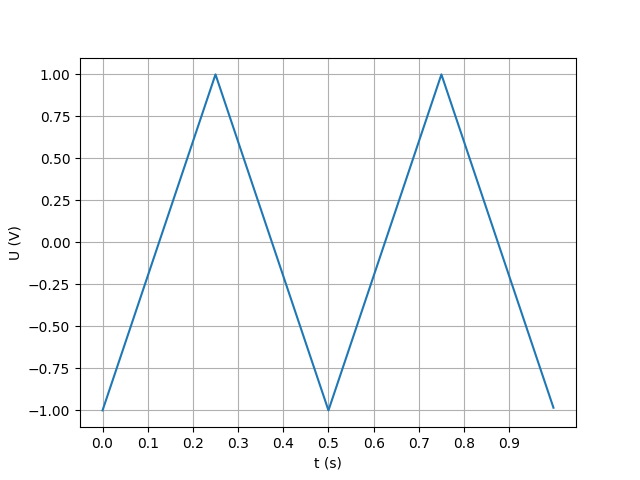
\includegraphics[height=0.3\textheight]{images/triangle.png}
    \end{center}
    
    \begin{itemize}
        \item La période de ce signal vaut : \trou{$T = \SI{0.2}{s}$}
        \item La fréquence de ce signal vaut : \trou{$f = \frac{1}{T}\SI{5}{Hz}$}
        \item  L'amplitude de ce signal vaut : \trou{$A = 1V$}
    \end{itemize}
    \pagebreak
    \section{Les appareils de mesures}
    \begin{figure}[h]
        \centering
        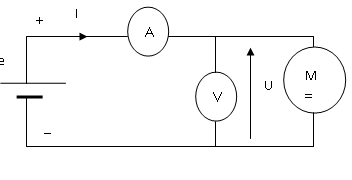
\includegraphics[height=0.2\textheight]{images/branchement.png}
        \caption{Branchement d'un voltmètre et d'un ampèremètre dans un circuit}
        \label{fig:branchement}
    \end{figure}
    
    \subsection{L'ampèremètre}
    L'ampèremètre sert à mesurer un courant électrique I. Il se place en \textbf{série} dans le circuit. 
    
    \subsection{Le voltmètre}
    Le voltmètre sert à mesurer une tension électrique (une différence de potentiel entre un point A et un point B du circuit). Il se place en dérivation entre A et B
\end{document}
